%\documentclass{beamer}
\documentclass[11pt,handout,pdf,hyperref={unicode}]{beamer}
\setbeamertemplate{navigation symbols}{}

\usepackage[T2A]{fontenc}
\usepackage[utf8]{inputenc}
\usepackage[english,russian]{babel}
\usepackage[style=authoryear]{biblatex}
\renewcommand*{\nameyeardelim}{\addcomma\addspace}
\graphicspath{ {images/} }
\DeclareGraphicsExtensions{.png,.pdf}
\addbibresource{custom.bib}
\usetheme{Warsaw}

\addtobeamertemplate{navigation symbols}{}{%
    \usebeamerfont{footline}%
    \usebeamercolor[black]{footline}%
    \hspace{10em}%
    \insertframenumber/\inserttotalframenumber
}

\newcommand{\backupbegin}{
   \newcounter{finalframe}
   \setcounter{finalframe}{\value{framenumber}}
}
\newcommand{\backupend}{
   \setcounter{framenumber}{\value{finalframe}}
}

%Information to be included in the title page:
\title[Тайм-трекинг на блокчейне]{Тайм-трекинг пользовательских действий на распределенной блокчейн-цепи}

\begin{document}

\author[Михаил Волхов, M3438]{
  Студент: Михаил Волхов, M3438\\
  Руководитель: Штукенберг Д.Г., тьютор кафедры КТ \\
  Рецензцент: Чепурной А.И, специалист, IOHK Research
}
\institute{Кафедра Компьютерных Технологий \\ факультет Информационных Технологий и Программирования \\ Университет ИТМО, Санкт-Петербург}
\date{16 мая 2017}

\frame{\titlepage}

\section{Введение и цели}

\subsection{Блокчейн и криптовалюты}

\begin{frame}
  \frametitle{Блокчейн, транзакция}

  Блок -- тело с транзакциями и заголовок, содержащий подписанный ключом
  эмитентом хэш предыдущего блока. Таким образом объединяются в цепочку. Право
  выпустить блок основывается на идее консенсуса (PoW или PoS).

  Адрес $Addr_i$ -- это хэш публичного ключа или скрипта. К
  транзакции прикладываются доказательства $\forall t \in txIn$.

  \begin{figure}[t]
  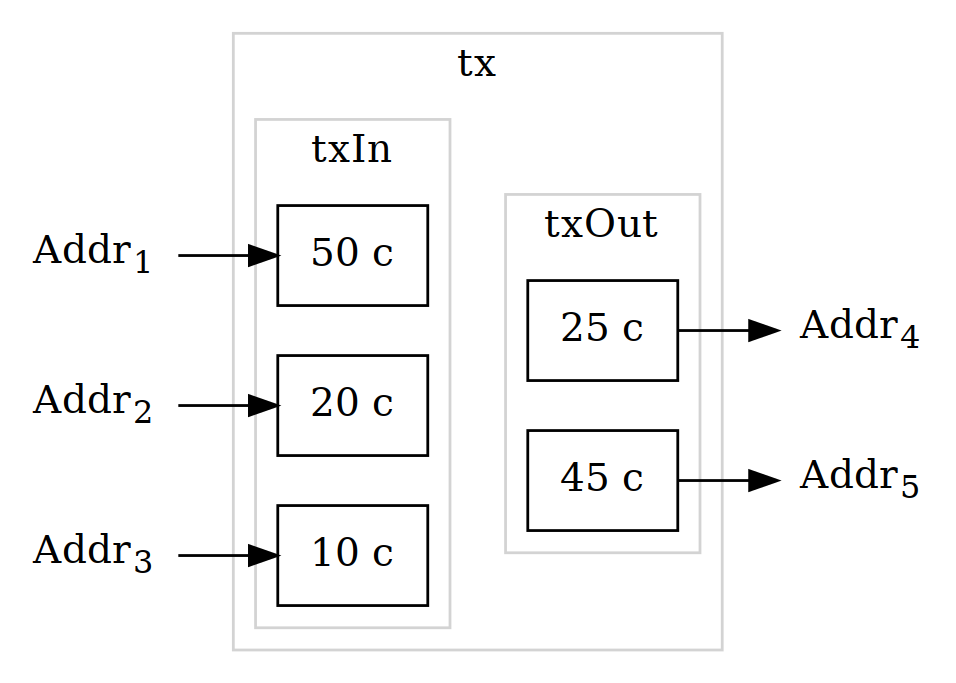
\includegraphics[scale=0.18]{tx_example}
  \centering
  \end{figure}
%  \begin{itemize}
%  \item Proof-of-work (PoW): стохастически, решение сложной
%    вычислительной задачи. Используется в Bitcoin \parencite{bitcoin}.
%  \item Proof-of-stake (PoS): выбор лидера с вероятностью,
%    пропорциональной его активам (stake).
%  \end{itemize}

\end{frame}

%\begin{frame}
%  \frametitle{Криптовалюта}
%
%  Тело блока содержит транзакции, переводящие средства с адресов на
%  адреса.
%\end{frame}

\begin{frame}
  \frametitle{Скриптинг и смарт-контракты}

  Деньги могут храниться не только на адресе публичного ключа, но и на скрипте.
  \begin{itemize}
  \item Адрес -- хэш скрипта
  \item Сам скрипт говорит, как можно снимать со скрипт адреса деньги.
  \item Адреса, с которых может снимать $n/m$ пользователей (multisig)
  \item Смарт-контракты, например аукционы в Hawk \parencite{kosba2016hawk}
    или DAO (decentralized autonomous organisations) в Ethereum.
  \end{itemize}
\end{frame}

\subsection{Тайм-трекинг}

\begin{frame}
  \frametitle{Тайм-трекинг}

  ПО, позволяющее ассоциировать активности с набором временных
  интервалов, а также анализировать эту статистику. Например, toggl,
  arbtt (автоматизированный, интеграция с X11), youtrack или org-mode.

  Пример тайм-трекинга задач в org-mode:
  \begin{figure}[t]
  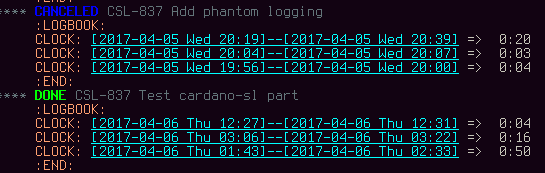
\includegraphics[scale=0.5]{org_mode_task}
  \centering
  \end{figure}
\end{frame}

\begin{frame}
  \frametitle{Открытые задачи}

  Что бы хотелось видеть:
  \begin{itemize}
  \item Трекинг мультипользовательские активностей -- знание о том,
    что группа пользователей выполняет активность
    совместно. Реализаций не существует.
  \item Формализованный и автоматизированный сбор статистики (но можно
    руками org-mode'ом, например, считая потраченное время по
    категориям задач).
  \end{itemize}
\end{frame}

\subsection{Поставленная задача}

\begin{frame}
  \frametitle{Идея/Мотивация}

  \begin{itemize}
  \item Мультипользовательские транзакции криптовалюты --
    мультипользовательские активности. В них можно выразить интервалы
    времени, тип активности. Сразу получаем подписи всех участников,
    что является кросс-подтверждением произведенного действия.
  \item По таким транзакциям в блокчейне можно вычислять
    \textit{рейтинг} пользователей с помощью смарт-контрактов;
    формализация правила выставления рейтинга -- \textit{контракт}.
  \item Рейтинг псевдопубличный, глобальный и финальный. Не зависит от
    того, с кем заключаешь контракт.
  \end{itemize}
\end{frame}

\begin{frame}
  \frametitle{Задача и примеры}
  Задача: разработать модификацию криптовалюты:
  \begin{itemize}
  \item Имеет функциональность тайм-трекинга.
  \item Мультипользовательские транзакции и контракты, выставление рейтинга.
  \item Не нарушает гарантий криптовалюты.
  \end{itemize}

  Примеры использования:
  \begin{itemize}
    \item Аггрегация глобального рейтинга фрилансеров, поддерживающая
      несколько бирж.
    \item Оптимизация семейных/дружеских отношений, обязанности и
      доказательства их (не)выполнения.
  \end{itemize}
\end{frame}

\section{Проделанная работа}

\subsection{База и модификации}

\begin{frame}
  \frametitle{Использованные технологии, изменения}

  В качестве базового протокола криптовалюты был выбран Ouroboros
  \parencite{ouroboros}: поддерживает удобную работу со временем
  (слоттинг), первый доказаный PoS алгоритм с сильными гарантиями
  безопасности.

  Предложена популярная модификация ``цветные монеты'', необходимая
  для кодирования информации о типе активности (используется поверх
  биткоина некоторыми кошельками, в RSCoin).
  \begin{itemize}
  \item Были добавлены монеты цвета рейтинга и действий.
  \item Показано, как сохранить гарантии протокола при интеграции.
  \end{itemize}
\end{frame}

\begin{frame}
  \frametitle{Цветные монеты, проблематика}

  Добавляем к монете тег цвета. Цвета конвертируются согласно графу
  конвертации $G_c$. Теперь валидация транзакции сложнее, чем
  проверить $\sum{in_i} \geq \sum {out_j}$. Задача: формализовать
  проблему и придумать алгоритм валидации цветной транзакции.

  \begin{figure}[t]
  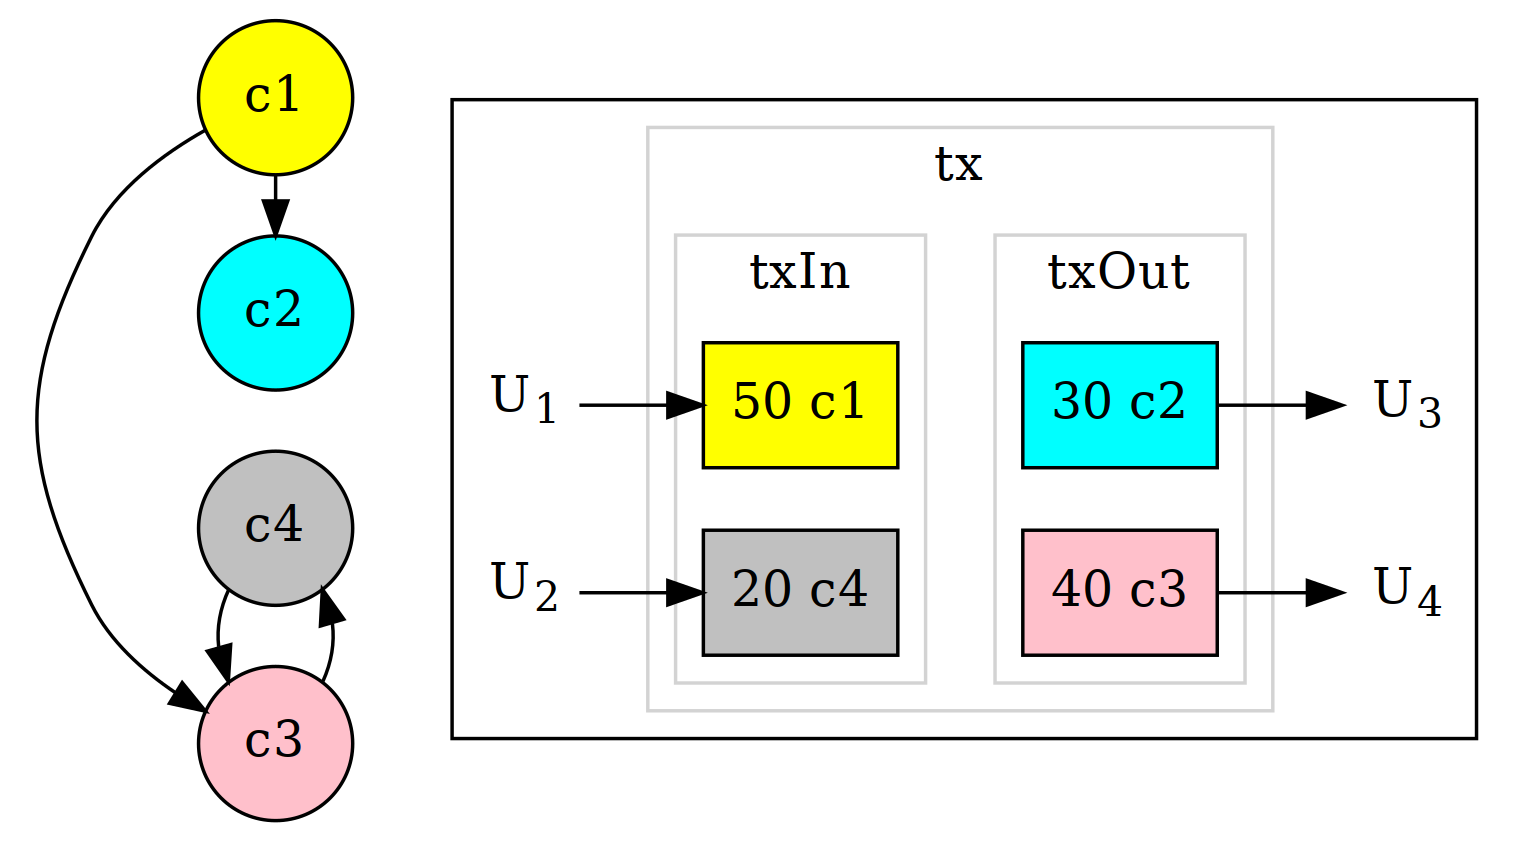
\includegraphics[scale=0.15]{pres_colortx.png}
  \centering
  \end{figure}

\end{frame}

\begin{frame}
  \frametitle{Валидация цветной транзакции}

  Формальное требование -- возможность разбить входы так, чтобы
  сопоставить их выходам:

  \[
  \exists H = \{H_i\}_i. \ MergeC(H) = MergeC(txIn) \wedge \forall c \in txOut . \ \exists i . \ C_g(H_i) = c
  \]


  Показано, как сводить задачу валидации к задаче о максимальном
  потоке. Вершины соответствуют входам одного цвета, ребра посередине
  строятся из $G_c$.

  \begin{figure}[t]
  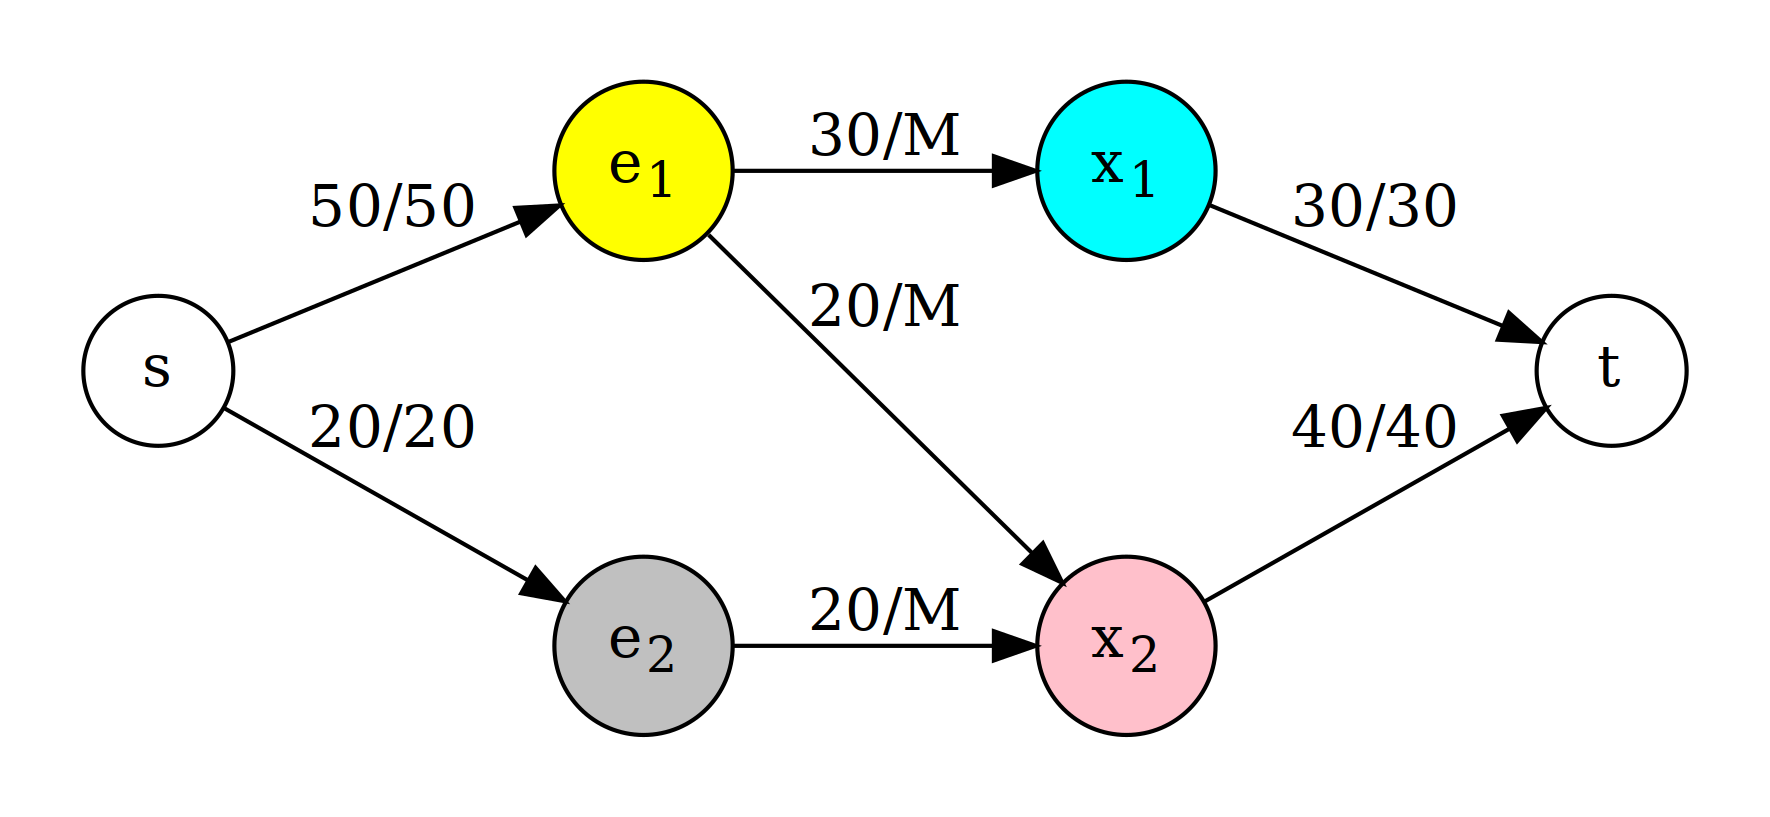
\includegraphics[scale=0.12]{pres_colortx_graph}
  \centering
  \end{figure}
\end{frame}

\subsection{Контракты и транзакции}

\begin{frame}
  \frametitle{Обязательства и транзакции} Контракт выражен как
  множество обязательств $rs = (supp, rec, \tau, act_i)$, где возможно
  накладывать временные ограничения в период контракта, а также
  выбирать множества исполнителей, которые допускаются к выполнению
  обязательства.

  Показан способ эмулировать тайм-трекинг с помощью транзакций криптовалюты.
  \begin{itemize}
  \item Первоначально использует реальную интервальную модель
    взаимодействия пользователя (пре-транзакцию) $[\tau_{start}, \tau_{end}]$.
  \item Конвертирует ее в транзакцию, кодируя все интервалы, не теряя
    необходимой информации.
  \item Решение использует схему вывода ключей Hierarchical
    Deterministic Keys / Ed25519.
  \end{itemize}
\end{frame}

\begin{frame}
  \frametitle{Выставление рейтинга и общий вид контракта}

  Формализована функция выставления рейтинга по условиям контракта и
  тайм-трек транзакциям:
  \begin{itemize}
  \item Максимальный рейтинг, если все обязанности
    удовлетворены. Минимальный, если ни одна.
  \item Учитывается важность пользователя для каждого обязательства
    $rs$ через представления $supp$ как коалиционную игру с
    использованием вектора Шепли.
  \item При подсчете штрафа учитывается количество времени уже
    потраченного на удовлетворение $rs$.
  \item Рейтинг пропорционален суммарному времени обязательств,
    скорректированному по важности пользователя.
  \end{itemize}

  Показан общий вид контракта как скрипта (темплейтная конфигурация,
  настраиваемые поля) и транзакция распределения рейтинга (использует
  функционал скриптинга).
\end{frame}

\begin{frame}
  \frametitle{Инфрастуктура}

  Предложен API для сервера, формирующего пре-транзакции и собирающего
  подписи для транзакций.

  Рассмотрены преимущества и недостатки централизованного и
  децентрализованного решения для физической реализации этого
  сервиса. Предложена модификация Kademlia, авторизованная стейком в
  Ouroboros, для избежания sybil атак.
\end{frame}

\section{Результаты}

\begin{frame}
  \frametitle{Результаты}

  Было предоставлено решение для тайм-трекинга поверх Ouroboros,
  содержащая в себе:
  \begin{itemize}
  \item Интеграция цветных монет, анализ, реальную схему.
  \item Обязанности, транзакции, контракт как скрипт.
  \item Функция выставления рейтинга.
  \item Физическая/программная модель.
  \end{itemize}
\end{frame}

\backupbegin
\section{}

\begin{frame}

  \begin{center}
    \Huge Вопросы?
  \end{center}

\end{frame}


\begin{frame}
  \frametitle{Почему блокчейн, а не централизованное?}

  Почему вообще блокчейн?
  \begin{itemize}
  \item Сервисов много, рейтинг -- один.
  \item Одна биржа труда сегодня, другая -- завтра. Блокчейн хранит историю.
  \item Решение ``из коробки''.
  \end{itemize}

  Почему конкретно блокчейн? (по сравнению с BFT алгоритмами
  \parencite{powbftquest})?:
  \begin{itemize}
  \item Открытость по отношению к участникам, полная децентрализация
    $\Rightarrow$ нет единого источника доверия.
  \item Отличное масштабирование по пользователям и узлам.
  \end{itemize}
\end{frame}

\begin{frame}
  \frametitle{Почему цветные монеты? }

  В представленном решении:
  \begin{itemize}
  \item Понятное и почти готовое решение (EPOBC, OAP, Colu),
    представленое в другой форме.
  \item Мнемонически простое и эффективное, сравнивая с другими
    способами кодирования информации о типе активности.
  \end{itemize}

  В общем смысле:
  \begin{itemize}
  \item Эмулировать другие ресурсы и другие типы валют (золото, нефть,
    акции).
  \item Отслеживать движение средств без необходимости парсинга всего
    блокчейна (напрямую из utxo).
  \end{itemize}
\end{frame}

\backupend

\end{document}
